\documentclass[11pt,fleqn]{article}
\linespread{1.3}
\usepackage{parskip}
\setlength{\parindent}{0pt} %no paragraph indentation
\setlength{\parskip}{2.1ex plus 0.2ex minus 0.2ex} %3x paragraph spacing
\usepackage{geometry}
\geometry{a4paper,left=30mm,right=25mm,top=20mm,bottom=20mm} %margin spacing
\usepackage{fancyhdr}
\pagestyle{fancy}
\fancyhf{}
\renewcommand{\headrulewidth}{0pt}
\rfoot{\thepage}

\usepackage[pdftex]{graphicx} %so that eps files may be included
\usepackage{amsmath}
\usepackage{amssymb}
\usepackage{amsthm}
\usepackage{float}

% Theorems, definitions etc.
\newtheoremstyle{defstyle}
  {10pt} % Space above
  {0pt} % Space below
  {} % Body font
  {} % Indent amount
  {\bfseries} % Theorem head font
  {.} % Punctuation after theorem head
  {0.5em} % Space after theorem head
  {} % Theorem head spec (can be left empty, meaning `normal')
\theoremstyle{defstyle}
\newtheorem{defn}{Definition}[section]

\begin{document}
%Title page
\begin{titlepage}

\center % Center everything on the page
 
%----------------------------------------------------------------------------------------
%	HEADING SECTIONS
%----------------------------------------------------------------------------------------

\textsc{\LARGE University of Pretoria}\\[1.5cm] % Name of your university/college
\textsc{\Large Department of Mathematics and Applied Mathematics}\\[0.5cm] % Major heading such as course name
\textsc{\large WTW 795: Essay}\\[3.5cm] % Minor heading such as course title

%----------------------------------------------------------------------------------------
%	TITLE SECTION
%----------------------------------------------------------------------------------------


\huge \textsc{Finite Element Approximation for Convection, Diffusion and Reaction systems in a Tubular Reactor} \\[3.5cm]
 
%----------------------------------------------------------------------------------------
%	AUTHOR SECTION
%----------------------------------------------------------------------------------------

\begin{minipage}{0.4\textwidth}
\begin{flushleft} \large
\emph{Author:}\\
St. Elmo Wilken % Your name
\end{flushleft}
\end{minipage}
~
\begin{minipage}{0.4\textwidth}
\begin{flushright} \large
\emph{Student Number:} \\
29034133 
\end{flushright}
\end{minipage}\\[2cm]

\begin{minipage}{0.4\textwidth}
\begin{center} \large
\emph{Supervisor:} \\
Prof. van Rensburg % Supervisor's Name
\end{center}
\end{minipage} \\[2cm]

%----------------------------------------------------------------------------------------
%	DATE SECTION
%----------------------------------------------------------------------------------------

{\large \today}\\[3cm] % Date, change the \today to a set date if you want to be precise

\vfill % Fill the rest of the page with whitespace

\end{titlepage}

%Abstract and Keywords
\begin{center}
\Large Finite Element Approximation for a Convection, Diffusion and Reaction System in a Tubular Reactor \\[0.5cm]
\large St. Elmo Wilken \\
29034133
\end{center}

\begin{abstract}
Insert abstract...
\end{abstract}

\textsc{\small KEYWORDS:} \small Finite Element Method, diffusion, convection, reaction, tubular reactor
\tableofcontents
\pagenumbering{gobble}

\newpage
\pagenumbering{arabic}
\section{Introduction}

\section{Model Derivation}
In this section the general convection, diffusion and reaction (CDR) continuum equation is developed. Furthermore, the accompanying energy balance necessitated by the reaction component of the resultant model is also derived. For the purposes of this project a tubular reactor geometry is assumed; thus the model is derived with respect to the (more natural) cylindrical coordinate system. 

\begin{defn}
Diffusion is the spontaneous mixing of molecules by random thermal motion. It gives rise to motion of a chemical species relative to the motion of the mixture.
\end{defn}

In the absence of other gradients, molecules of a single species will always diffuse from regions of higher concentration to regions of lower concentration. This concentration gradient results in a molar flux of the species.

\begin{defn}
For species A the molar flux is denoted by $\mathbf{W}_A$ and has units of $\frac{moles}{time \times area}$. The molar flux is a vector quantity and can be expressed as $\mathbf{W}_A = W_A|_r \mathbf{e}_r + W_A|_\theta \mathbf{e}_\theta + W_A|_z \mathbf{e}_z$ in cylindrical coordinates. The molar flow rate is related to the molar flux and cross-sectional area by $F_A|_i = A_c|_i \times W_A|_i$ where $i$ indicates the component of interest. 
\end{defn}

The basis of the model's derivation rests on the conservation of mass principle. A consequence of this assumption is the mole balance: barring a reaction, the number of moles of a species is conserved within a given control volume. The mole balance for the reacting species A is derived with reference to the control volume depicted in Figure \ref{fig_vol_element}.

\begin{figure}[H] 
\centering
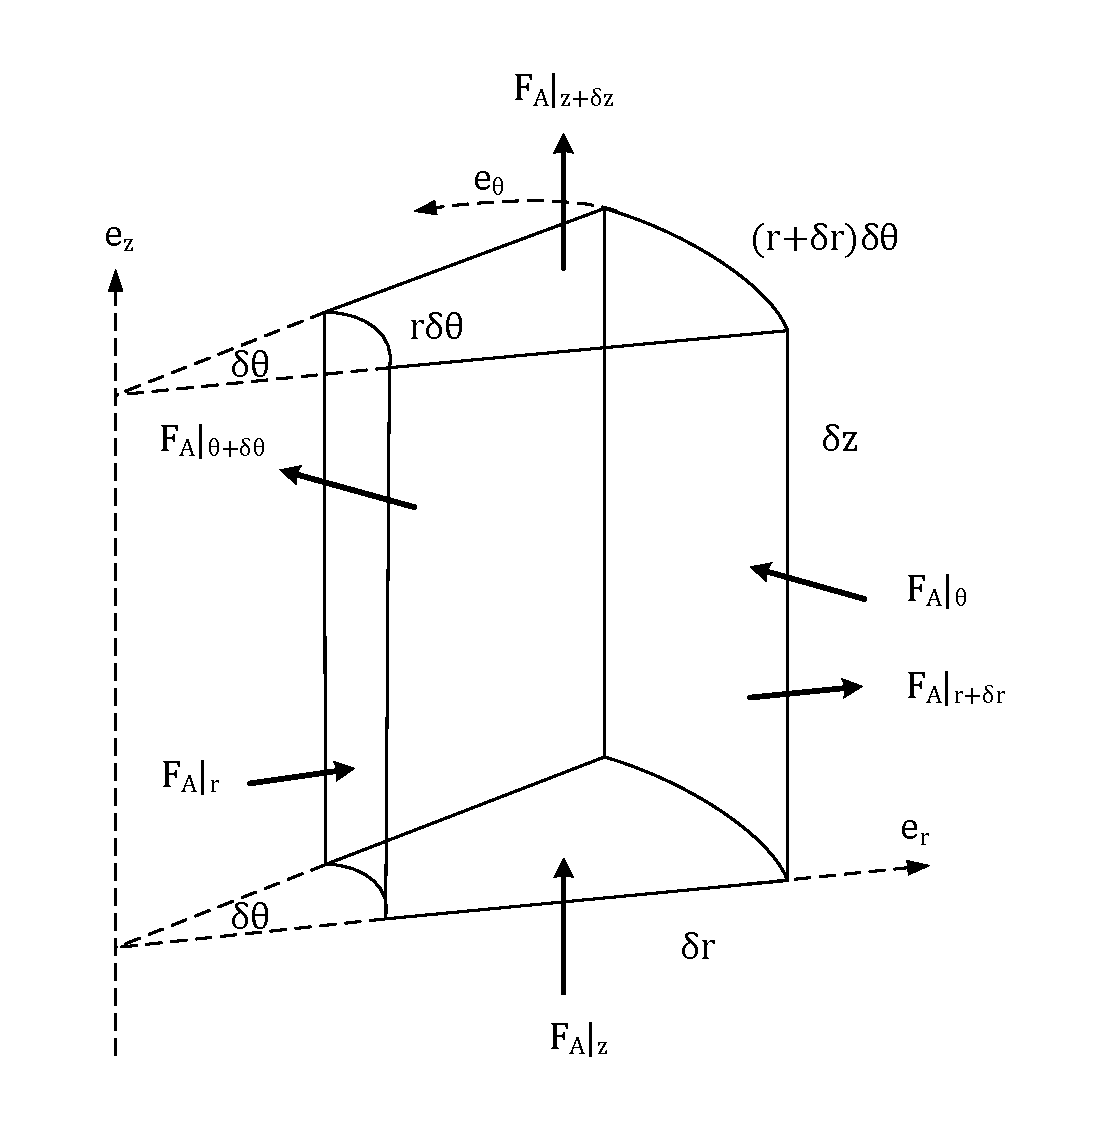
\includegraphics[scale=0.5]{volume_element}
\caption{Control volume element for a tubular reactor} 
\label{fig_vol_element}
\end{figure}

The mole balance is shown in (\ref{eq_mole_balance}) where $r_A$ indicates the generation or consumption of species A due to reaction and $C_A$ is the concentration of species A in the mixture. The term on the right hand side of (\ref{eq_mole_balance}) represents the accumulation of species A in the control volume ($\delta V$).
\begin{equation}
\sum_{i=r, \theta, z}[F_A|_i(i) - F_A|_i(i+\delta i)] + r_A \delta V = \delta V \frac{\partial C_A}{\partial t}
\label{eq_mole_balance}
\end{equation}

Consider the molar flow rate in the $\mathbf{e}_r$ direction. By using the definition of molar flux and the first order Taylor series expansion of $F_A|_r(r+\delta r)$ we have (\ref{eq_far}).
\begin{equation}
\begin{aligned}
F_A|_r(r) &= W_A|_r(r) r \delta \theta \delta z \\
F_A|_r(r+\delta r) &= (W_ A|_r(r) + \frac{\partial W_A|_r(r)}{\partial r} \delta r)(r+\delta r)\delta \theta \delta z
\end{aligned}
\label{eq_far}
\end{equation}
Neglecting higher order terms we have (\ref{eq_far2}).  
\begin{equation}
F_A|_r(r) - F_A|_r(r+\delta r)  = - (W_ A|_r(r)  + \frac{\partial W_A|_r(r)}{\partial r}r) \delta r \delta \theta \delta z
\label{eq_far2}
\end{equation}
In a similar manner, consider the molar flow rate in the $\mathbf{e}_\theta$ direction. By again using the definition of molar flux and the first order Taylor series expansion of $F_A|_\theta(\theta+\delta \theta)$ we have (\ref{eq_fat}).
\begin{equation}
\begin{aligned}
F_A|_\theta(\theta) &= W_A|_\theta(\theta) \delta r \delta z \\
F_A|_\theta(\theta + \delta \theta) &= W_A|_\theta(\theta) \delta r \delta z + \frac{\partial W_A|_\theta(\theta)}{r \partial \theta}\delta \theta\delta r \delta z
\end{aligned}
\label{eq_fat}
\end{equation}
Consequently we have (\ref{eq_fat2}).
\begin{equation}
F_A|_\theta(\theta) - F_A|_\theta(\theta + \delta \theta) =- \frac{\partial W_A|_\theta(\theta)}{r \partial \theta}\delta \theta\delta r \delta z
\label{eq_fat2} 
\end{equation}
Finally, consider the molar flow rate in the $\mathbf{e}_z$ direction. By using the definition of molar flux, the first order Taylor series expansion of $F_A|_z(z+\delta z)$, approximating the cross-sectional area normal to $\mathbf{e}_z$ in Figure \ref{fig_vol_element} as a trapezium and neglecting higher order terms, we have (\ref{eq_faz}).
\begin{equation}
\begin{aligned}
F_A|_z(z) &= W_A|_z(z) r \delta r \delta \theta \\
F_A|_z(z + \delta z) &= W_A|_z(z) r \delta r \delta \theta + \frac{\partial W_A|_z(z)}{\partial z}r \delta z \delta r \delta \theta
\end{aligned}
\label{eq_faz}
\end{equation}
Consequently we have (\ref{eq_faz2}).
\begin{equation}
F_A|_z(z) - F_A|_z(z + \delta z) = - \frac{\partial W_A|_z(z)}{\partial z}r \delta z \delta r \delta \theta
\label{eq_faz2}
\end{equation}
Substituting (\ref{eq_far2}), (\ref{eq_fat2}) and (\ref{eq_faz2}) into (\ref{eq_mole_balance}) results in (\ref{eq_mb2}). Note that for sufficiently small $\delta r$ we have $\delta V \approx r \delta \theta \delta r \delta z$.
\begin{equation}
- (W_ A|_r(r)  + \frac{\partial W_A|_r(r)}{\partial r}r) \delta r \delta \theta \delta z - \frac{\partial W_A|_\theta(\theta)}{r \partial \theta}\delta \theta\delta r \delta z - \frac{\partial W_A|_z(z)}{\partial z}r \delta z \delta r \delta \theta + r_A \delta V = \delta V \frac{\partial C_A}{\partial t}
\label{eq_mb2}
\end{equation}

Dividing through by $r \delta \theta \delta r \delta z$ results in (\ref{eq_mb3}) which is equivalent to (\ref{eq_mb4}).
\begin{equation}
-\frac{1}{r} W_A|_r - \frac{\partial W_A|_r}{\partial r} - \frac{1}{r^2}\frac{\partial W_A|_\theta}{\partial \theta} - \frac{\partial W_A|_z}{\partial z}+ r_A  = \frac{\partial C_A}{\partial t}
\label{eq_mb3}
\end{equation}
\begin{equation}
-\frac{1}{r} \frac{\partial (rW_A|_r)}{\partial r} - \frac{1}{r^2}\frac{\partial W_A|_\theta}{\partial \theta} - \frac{\partial W_A|_z}{\partial z}+ r_A  = \frac{\partial C_A}{\partial t}
\label{eq_mb4}
\end{equation}

It is now necessary to make modelling assumptions. Firstly, we will neglect any variations in the rotational direction (modelled by assuming $\frac{\partial W_A|_\theta}{\partial \theta} \approx 0$).

Secondly, we assume that Fick's Law is valid, that the diffusivity ($D_{AB}$) is constant and that the total concentration of the system is constant. This last assumption limits us to considering only reactions which conserve the total number of moles e.g. $A \rightarrow B$ or $A + B \rightarrow 2C$ etc..

Thirdly, we assume that the convection in the radial direction is negligible and that the velocity profile of molar flow in the axial direction only varies in the radial direction ($U(z,r)=U(r)$). These assumptions are not particularly strong but nevertheless simplify the model considerably. The resultant constitutive equations are shown in (\ref{eq_fick}).  
\begin{equation}
\begin{aligned}
W_A|_z &= -D_{AB}\frac{\partial C_A}{\partial z} + C_A U(r) \\
W_A|_r &= -D_{AB}\frac{\partial C_A}{\partial r}  
\end{aligned}
\label{eq_fick}
\end{equation} 
Substituting (\ref{eq_fick}) into (\ref{eq_mb3}) results in the model we will be using for this project (\ref{eq_cdr}).
\begin{equation}
D_{AB}(\frac{1}{r}\frac{\partial}{\partial r}(r\frac{\partial C_A}{\partial r}) + \frac{\partial^2 C_A}{\partial z^2}) - U_z\frac{\partial C_A}{\partial z} + r_A = \frac{\partial C_A}{\partial t}
\label{eq_cdr}
\end{equation}

Up to now not much has been said about the reaction term $r_A$.

%References
\newpage
\bibliographystyle{plain}
\bibliography{research}

\end{document}